\chapter{智能会话系统}{Toward Intelligent Dialgoue}

       本文研究的其中一个长远目标便是结合前文提到的各项自然语言处理和逻辑推理技术,构建一个能较好地与人交流沟通的智能会话系统,此系统将接收到的人类话语转化成逻辑表达形式,并且结合系统本身的动机和情感状态,经过一定的解析和逻辑推理,从而得到想表达的内容的逻辑表达形式,最后将这些逻辑表达式再转化成自然语言回应给谈话对象。
       本章将重点介绍这样的智能会话系统(以下简称“CogDial”)的系统架构,该系统基于前面章节描述的自然语言理解和自然语言生成的相关技术,并通过OpenCog的核心子系统(主要是PLN和OpenPsi)来控制其对话结构和表达方式。该CogDial系统能够灵活地理解和处理具有不同程度的复杂性和智能性的人类言语行为。创建一个完全符合人类标准的人工智能对话系统无疑是一个精彩的挑战,但似乎在当前的科学技术水平下,也无疑是一个非常困难的研究项目。 相对于目前主流的基于规则或者基于统计的对话系统,我们这里提出的CogDial架构引入目标驱动的逻辑推理和情感控制等,显然表现更智能些,但还不足以完全达到符合人类智能标准。这样一个介于目前相关研究水平和完全人类水平之间的对话系统可以看做是构建更人性化的对话系统的一个重要步骤,或者看做是使用更可行的研究方法在人机对话系统上集成更多的功能,而不是一味地去盲目追求达到人类水平的目标。本着这样的理念,说的更具体点,我们CogDial的目标不是精确类似人类的对话,而是具备通用认知能力、情感表达能力、能合理结合语用和经验的智能会话系统。
         CogDial的初步预期目标主要是实现面向游戏角色和人性机器人的对话系统,但同样的研究思路也完全能应用在基于文本的对话系统,例如智能对话搜索接口。我们分阶段来实现这样的系统,以一个相对小而简单的系统为起点,通过不断改进和完善,以及结合系统本身的自学习和认知能力,最终实现一个在一定程度上接近人类水平的系统。目前,我们的系统还没有达到最终的水平,但基本框架已经到位。除此之外,我们构建了一个基于超图匹配的问答系统的原型,该问答系统使用前文提到的自然语言理解技术将自然语言转换成以超图表示的语义逻辑形式,利用基于超图匹配的动态编程算法,从而在问答语料库中找到最适合问题的答案来响应用户查询。

\section{基于Psi的对话控制}{Applying the Psi model to Dialogue Control}
构建一个完整能运作的智能对话系统,除了需要前文提到的各项关键技术, 宏观规划(以下称为“Marcoplanning”)也是必不可少的部分。从言语行为理论来看,宏观规划可以看成是一个可以规划以下两点的工具:1)在哪个时间点发生哪些言语行为,2)使用哪些内容去封装这些言语行为。宏观规划更多的是从语用和推理方面出发,淡化语义或语法(或者音韵词汇等)的限制。
      CogDial智能对话系统中的宏观规划涉及到了OpenCog中的情感动机计算模型OpenPsi,因此,在本节我们会首先给出OpenPsi的高度概括,侧重于介绍其在自然语言会话系统中应用的可行性。

\subsection{Psi模型中的动机行为}{The Psi Model of Motivated Action}
       为了更好的解释OpenPsi,我们需要从Psi和MicroPsi谈起,Psi是由德国心理学家Dietric Dorner提出的情感认知动机理论模型 \cite{Dorner2002},将情感与智能体的需求和动机相联系。{\bf MicroPsi} \cite{Bach2009},是一个基于Psi理论的一个开源的智能认知体系结构,实现了Psi理论中的动机、情感以及智能的关联模型,并在一些实用控制应用以及简单虚拟世界里的智能体上进行测试。MicroPsi在全面性以及神经科学和心理学依据方面做得非常出色,但是该认知体系结构在可扩展性上存在不少问题, \cite{EGI1}中,有人认为,MicroPsi目前使用的算法在学习和推理上不大可能被扩展或规模化。
       OpenCog受Psi理论中的动机和情感模型的启发,借鉴了很多MicroPsi的基本实现方法,实现了类似的情感动机模型OpenPsi。虽然OpenPsi和MicroPsi在一定程度上很相似,但两者 还是存在着很大的不同。比如,两者使用了完全不同的知识表达方式, MicroPsi则使用了类似神经元的“quad”来表示知识,每一个quad包括5个神经元,其中一个是核心神经元,其他4个描述与核心神经元的“前/后”或者“部分/整体”等关系。OpenPsi使用了本文第三章中介绍的OpenCog的基于超图的知识表示,显然是一种更灵活和通用的知识表示方式。 MicroPsi目前还是注重底层的智能的实现,还未开始着手高层的智能处理,如自然语言处理和抽象逻辑推理。
在本节对Psi和MicroPsi的概述中,我们主要介绍其在OpenCog被应用的部分,主要是处理动机、行为和目标的框架模型。
Psi理论中的动机机制可参考图\ref{fig:Psi},从下往上看,不难发现Psi的动机机制从能激发智能体的需求出发。对于动物来说,该需求可以是食物、水、保护自己的孩子、社交需求、求新等等;对于智能机器人来说,该需求可能是电源、 完整性(保护身体完整Integrity)、确定性(了解和熟悉环境的需求Certainty)、认知需求、心里成长等等;对于智能对话系统来说,该需求可以包括收集相关信息、取悦谈话对象、使会话保持新颖不枯燥等。
Psi理论特别指出了两种相当抽象的需求,并认为他们是心理学上的最基本需求[见图XX] 


\begin{itemize}
\item 能力需求(Competence):  智能体能有效实现某种强烈欲望的需求
\item 确定性需求(Certainty):智能体了解和熟悉环境的需求 
\end{itemize}

每种需求都有一定的偏好范围或目标范围,随着时间和环境(包括智能体自身)的不断变化,智能体的需求也在不断地变化。 当需求水平落在相应的目标范围时,
称作该需求被满足,否则需求不被满足。我们可以将智能体视为一个目标驱动的
系统,其主要任务就是尽可能让所有这些需求都被满足。而当某一需求不被满足
时,智能体会有一种试图将该需求水平恢复到偏好范围内的愿望,这种愿望便构
成了动机。

\begin{figure}[htb]
\centering
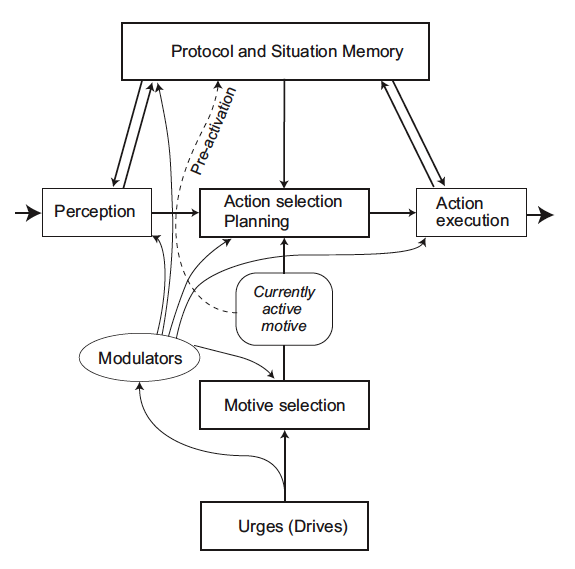
\includegraphics[width=11cm]{figures/Psi.png}
\caption{High-Level Architecture of the Psi Model}
\label{fig:Psi}
\end{figure}

%%%%%%%%%%%%%%%%%%%%%%%%%%%%%%%%
\subsection{Emotion and Personality in the Psi Model}
%%%%%%%%%%%%%%%%%%%%%%%%%%%%%%%%

%%%%%%%%%%%%%%%%%%%%%%%%%%%%%%%%
\section{OpenPsi:OpenCog中的基于Psi的动机性行为模型}{OpenPsi: Psi-Based Motivated Action in OpenCog}
%%%%%%%%%%%%%%%%%%%%%%%%%%%%%%%%

本节将介绍OpenCog中如何集成基于Psi的动机性行为模型,使其能为我们的智能会话系统CogDial提供能用于动机性行为选择机制。

%%%%%%%%%%%%%%%%%%%%%%%%%%%%%%%%
\subsection{ Action Selection in OpenCog}
%%%%%%%%%%%%%%%%%%%%%%%%%%%%%%%%

正如Stan Franklin\cite{Franklin1995}指出的,智能的{\it 智能体}的本质在于它可以做事,还可以采取{\it 行为}。我们的智能会话系统CogDial中的行为选择会涉及OpenCog中所采用的行为选择机制\cite{EGI2},因此本章节首先简单介绍该行为选择机制的基本思路,以及Psi的变体模型如何在OpenCog中处理动机(包括情感、驱动、目标等)和对行为选择的指导。

OpenCog中的行为选择机制的关键部分在于:

\begin{itemize}
\item 行为选择器(Action Selector)根据当前环境选择可能帮助实现重要目标的程序
\begin{itemize}
\item {\it 例如:} 假设当前十分重要的目标是取悦谈话对象,一旦谈话对象问了问题,那么回答该问题会被评估为很可能可以达到“取悦谈话对象”的目标的程序。
\end{itemize}

\item 为了支持行为选择器,OpenCog设立了这样的蕴含式$Context \& Procedure \rightarrow Goal$,其中上下文(Context)是一个被赋值于智能体处境的谓词,在智能对话系统中,我们视为语境。

\begin{itemize}
\item {\it 例如:} 如果Bob请求智能体(智能会话系统)去写一段话,又假设该智能体知道Bob非常执着,那么该蕴含式可以被用成:
 \begin{itemize}
 \item ``Bob命令执行 X''  and ``执行 X''  $\rightarrow$ ``取悦 Bob''  $<.9,.9>$
 \end{itemize}

\item {\it 例如:} 如果智能体想说服谈话对象相信某个陈述X,那么该蕴含式可以被用成:
 \begin{itemize}
 \item ``告诉Bob我为什么相信X是正确''  and ``我想要说服Bob相信X是正确''  $\rightarrow$ ``满足度''  $<.9,.9>$
 \end{itemize}

\end{itemize}
\item 这些蕴含式的真值可以根据经验和推理来赋值。
\begin{itemize}
\item {\it 例如:} 第一个例子中的蕴含式的真值可以根据经验来赋值,即通过与记忆里Bob给出指令相关的情节来判断
\item {\it 例如:} 也能根据推理来赋值,即根据与Bob相似的个体给出指令的经验来类推,或结合Bob本人的明确表达,和Bob的自我描述通常合理的知识来推断
\end{itemize}

\item 重要值(Importance Value)可以通过经济注意力分配
Importance values are propagated between goals using economic attention allocation (and, inference is used to learn subgoals from existing goals).  This is an aspect we have not yet explored in practice in CogDial, but we believe it will be helpful for achievement of more sophisticated dialogue behavior.
\begin{itemize}
\item {\it 例如:} If Bob has told the agent to do X, and the agent has then derived (from the goal of pleasing Bob) the goal of doing X, then the ``please Bob''  goal will direct some of its currency to the ``do X''  goal (which the latter goal can then pass to its subgoals, or spend on executing procedures)
\end{itemize}
\end{itemize}

%%%%%%%%%%%%%%%%%%%%%%%%%%%%%%%%
\subsection{Psi in OpenCog}
%%%%%%%%%%%%%%%%%%%%%%%%%%%%%%%%

%%%%%%%%%%%%%%%%%%%%%%%%%%%%%%%%
\subsection{Goals in OpenCog}
%%%%%%%%%%%%%%%%%%%%%%%%%%%%%%%%

%%%%%%%%%%%%%%%%%%%%%%%%%%%%%%%%
\subsection{Execution Management}\label{Execution Management}
%%%%%%%%%%%%%%%%%%%%%%%%%%%%%%%%

%%%%%%%%%%%%%%%%%%%%%%%%%%%%%%%%
\section{The CogDial Dialogue System Architecture}
%%%%%%%%%%%%%%%%%%%%%%%%%%%%%%%%

下面我们来介绍基于上述的目标控制体系的智能会话系统CogDial的系统框架。目前该系统只能处理英文对话,接下来章节中的对话的例子基本按照英文的习惯举的例子,可能不太适合中文的习惯,但是该系统的所采用的技术和理论基础都是完全适合中文的。CogDial主要采用了以下技术:

\begin{itemize}
\item  基于OpenPsi以及相关OpenCog机制的宏观规划(Macroplanning)
\item  本文第4章描述的句法分析和语义关系及逻辑关系抽取的自然语言理解技术
\item  本文第5章描述的微观规划(Microplanning)和表层生成的自然语言生成技术
\item  专门设计的符合智能会话系统的“言语行为规划器”集合,这些言语行为规划器将用于:
\begin{itemize}
\item 在OpenPsi的控制机制下,结合当前的语境,激活相应的言语行为规划器
\item 收集相关内容,生成能关联Microplanner的Atoms
\item  调用一系列的认知机制(包括用于逻辑推理的PLN),选择相关的Atoms发送到Microplanner
\end{itemize}
\end{itemize}

%%%%%%%%%%%%%%%%%%%%%%%%%%%%%%%%
\subsection{针对对话控制的OpenPsi的配置}{Configuring OpenPsi for Dialogue Control}
%%%%%%%%%%%%%%%%%%%%%%%%%%%%%%%%

基于Psi的基本框架,我们选择了以下的具体需求用来指导我们的对话系统的行为:
\begin{itemize}
\item 社交需求(Affiliation):与他人互动,希望被其他成员接纳的需求;取悦谈话对象可以视为此目标的一个特例
\item 能力需求(Competence):通过对话达到某种目标的需求,衡量言语表达方式的指标
\item 确定性需求(Certainty):智能体对自身语境的了解需求,特别是对目标的了解需求
\item 新颖性需求(Novelty):维持智能的会话而不是简单重复的问答会话。
\end{itemize}

CogDial中的对话控制主要通过不同的需求来选择相应的言语行为规划器,因此,在选择言语行为规划器前,我们需要知道当前状态下上述每种需求的被满足的程度。鉴于目前的CogDial系统的有限能力,为了能更好地实现一个面向集成认知体系的智能会话系统框架,我们将上述的几项需求做了更具体化的定义:

\begin{itemize}
\item 社交需求(Affiliation):我们对该需求进行了下面三种满足程度:
\begin{itemize}
\item 当对话系统正在与人或者其他智能体进行会话时,该需求在一定程度上被满足;
\item 当系统正与多个人或智能体进行会话时,该需求被满足的程度提升;
\item  当该系统的会话内容都属于积极向上的时候(通过情感分析技术实现),该需求被满足的程度达到最高。
\end{itemize}
\item 能力需求(Competence):此项需求需要通过OpenCog来评估。简单来说,对每一个目标,OpenCog记录着会话系统在过去完成该项目标的程度,然后根据当前的不同目标所占的权重,我们可以通过以下公式估算该需求被满足的程度(首先针对每一个目标,计算目标权重*能达到该目标的概率,然后求总)。当然计算目标被完成的程度,还应该考虑实现目标的语境等因素,目前我们的系统更注重构建一个智能会话系统框架,因此在语境无关的假设下来衡量目标被实现的程度。
\item 确定性需求(Certainty):如果会话系统正在和一个陌生人对话,或者系统无法理解大量被提及的单词或概念,那么当前的确定性需求被满足的程度就会降低。如果系统获取了新的可靠知识,那么该需求被满足的程度就会增加。
\item 新颖性需求(Novelty):我们定义了以下几种方式来增加智能绘画系统对新鲜度需求的满足程度值:
\begin{itemize}
\item 多和不同的人类或智能体会话;
\item 谈论新的话题或引入新的词汇和概念;
\item 学习新的可靠信息( OpenCog推理得出的新的置信度高的知识存储的载体原子(Atoms))
\end{itemize}
\end{itemize}

基于上述目标需求的智能会话系统,除了需要结合前文所述的OpenPsi的框架理论,以及本文描述的自然语言理解和生成的相关工具之外,还需要有以下模块:
\begin{itemize}
\item 制定一组能被特定目标需求激活的对话控制程序
\item 建立目标和相应去实现目标的行为之间的关联,可通过相关规则来实现,也可以通过强化学习来实现,我们系统框架采用两种结合的方法,但目前的系统还是以规则关联为主。
\end{itemize}
  

%%%%%%%%%%%%%%%%%%%%%%%%%%%%%%%%%%%%%%%%%%%%%%%%%%%%%%%%%%%%%%%
\subsection {言语行为规划器}{Speech Act Schema}
\label{sec:SAS}
%%%%%%%%%%%%%%%%%%%%%%%%%%%%%%%%%%%%%%%%%%%%%%%%%%%%%%%%%%%%%%%


“言语行为规划器”(Speech Act Schema)是CogDial的一个核心设计, 每个言语行为规划器里包含一种特定的言语行为(Speech Act),以及与该言语行为对应的特定的认知行为(Cognitive Procedure)。每种言语行为规划器都能在不同情况下被激发调用。对于言语行为规划器的选择,我们采用OpenCog中的OpenPsi的动机驱动模块来执行。
    CogDial的总体规划是针对本文第 \ref{chap:litreview}章综述里提到的42种SWBD-DAMSL言语行为 \cite{Twitchell2004},实现相应的言语行为规划器。 CogDial目前只实现了42种中的部分言语行为对应的言语行为规划器。另一方面,CogDial中的言语行为规划器的设计也绝不局限于这42种言语行为,CogDial实现了一些言语行为规划器能对应这42种中的某两种或多种言语行为,比如我们利用真值回答规划器(TRUTH VALUE ANSWER schema)来同时关联其中的YES QUESTION和NO QUESTION,从而可以将一般疑问句的回答根据真值的大小延伸到“可能”“不确定”“可能不”等,而不仅仅是局限于回答“是”或者“不是”。CogDial还根据智能体的具体情况拆分了这42种中的某些言语行为,例如,我们针对言语行为“STATEMENT” 实现了两个不同的言语行为规划器:回应声明以及智能体自发的用于表达其自身状态和想法等的声明。
总的来说,本文虽然没有完全照搬SWBD-DAMSL的言语行为分类,但是,该分类体系是来源于对大量人类会话的进行具体分析后的实验结果,也在具体的会话分析和抽象的言语行为理论之间架起了桥梁,使得抽象的言语行为理论在机器上实现变得可行,因此,SWBD-DAMSL的言语行为分类体系还是很有借鉴价值的。
要实现上述的言语行为规划器,每一个言语行为都会引发一个相应的认知行为,也就是说,每一个言语行为都会触发调用一段程序;而这样的机制正好符合OpenCog里的 GroundedSchemaNode的用法。GroundedSchemaNode是OpenCog的超图知识库里的一种节点类型,通常被封装在ExecutionOutputLink里,连接着一段代码(一般情况下是Scheme或者Python编写的代码)的名称。该代码可以通过ExecutionOutputLink被触发和执行。因此,鉴于这样的执行机制,我们可以通过对每个言语行为规划器定义一个GroundedSchemaNode来实现言语行为规划器。这样的设计方案可以减少冗长复杂的代码块,而直接通过OpenCog中统一又通用的Atomspace的基本操作方法来管理和执行复杂的言语行为规划器。另外,这样的机制也能很容易调用知识库Atomspace之外的复杂程序,从而得到很好的扩展性,也为言语行为规划器的扩展研究搭建了个很好的平台。例如,我们可以通过调用外部程序将逻辑推理系统PLN的前向或者后向推理应用到言语行为规划器中,使其能实现自适应学习,不断完善言语行为规划器。本文后面会进一步讨论这样的扩展。
每一个言语行为规划器的输入是一个被叫做对话节点(DialogueNode),DialogueNode是可以表示一方或者多方之间的会话交互的节点类型。DialogueNode可以有不同话语节点(UtteranceNodes)作为成员,在实现方式上,DialgoueNode通过MemberLinks指向不同的UtteranceNodes。而UtteranceNode则可以关联以下不同类型的节点:
\begin{itemize}
\item 关联一个或多个文本节点(TextNode)、句子节点(SentenceNode)或者短语节点(PhraseNode),则表示输入的话语内容来自一个或者多个文本、句子或者短语。
\item  关联一个声音节点(SoundNode),则表示该话语来自外界声音。
\item  关联指向说话者的Link。
\item  关联指向对话语的补充信息的Links,这些补充信息可以是该话语的言语行为类型、与该话语相联系的情感等。
\item  关联指向产生话语的言语行为规划器,用于响应是什么触发该话语。
\item  关联一个或多个解析节点(InterpretationNode),这些解析节点可以是用来解析话语的语义和语用信息。
\end{itemize}
言语行为规划器的输出是连接了一系列相关联Atoms的SetLink,该输出会送入本文\ref{chap:generation}中描述的微观规划和表层生成等工具,从而产生相应的自然语言来回应输入的内容。言语行为规划器还会将输出的话语关联到产生该话语的DialogueNode,这样不仅仅是记录了会话的内容,还能用于智能体的强化学习和提高智能体的各种需求的满足度。
下面通过一个例子来解释上述的实现过程。假设有下面的简单对话:
\begin{verbatim}
Ruiting: How are you doing?
CogDial: I am fine
\end{verbatim}
这个简单的对话可用以下的Atoms来表示:

{\tt\begin{small}\begin{lstlisting}

MemberLink
	UtteranceNode [555]
	DialogueNode [123]
	
MemberLink
	UtteranceNode [666]
	DialogueNode [123]
	
EvaluationLink
	PredicateNode "say"
	ConceptNode "Ruiting"
	UtteranceNode [555]

EvaluationLink
	PredicateNode "say"
	ConceptNode "me"
	UtteranceNode [666]
		
EvaluationLink
	PredicateNode "Textual Content"
	UtteranceNode [555]
	SentenceNode "How are you doing?"
	
EvaluationLink
	PredicateNode "Textual Content"
	UtteranceNode [555]
	SentenceNode "I am fine."
	
EvaluationLink
	PredicateNode "Utterance Type"
	UtteranceNode [555]
	ConceptNode "Interrogative"
	
EvaluationLink
	PredicateNode "Utterance Type"
	UtteranceNode [666]
	ConceptNode "Declarative"
	
AtTimeLink
	UtteranceNode [555]
	TimeNode "22:15:33 12/06/2014"
	
AtTimeLink
	UtteranceNode [666]
	TimeNode "22:15:47 12/06/2014"
	
EvaluationLink
	PredicateNode "Interpretation"
	UtteranceNode [555]
	InterpretationNode [22]
	
EvaluationLink
	PredicateNode "Interpretation"
	UtteranceNode [666]
	InterpretationNode [33]
	
	
MemberLink
	EvaluationLink
		PredicateNode "doing"
		ListLink
			ConceptNode "you"
			VariableNode "var1"
	InterpretationNode [22]
	
	
MemberLink
	InheritanceLink
		ConceptNode "I"
		ConceptNode "fine"
	InterpretationNode [33]
	
ExecutionLink
	GroundedSchemaNode "polite_banter.scm"
	ListLink
		UttteranceNode [555]
		DialogueNode [123]
	UtteranceNode [666]

\end{lstlisting}\end{small}}

其中的命题也可以有多种选择,例如:

{\tt\begin{small}\begin{lstlisting}
EvaluationLink
	PredicateNode "Conversation Partner"
	DialogueNode $D
	$X
\end{lstlisting}\end{small}}

该命题为真,当且仅当,$X是$D其中一个话语的发言人。


\section{Initial Speech Act Schema and their Linkage to Goals and Contexts}


在 \cite{Twitchell2004}, 中,Twitchell和Nunamaker根据Searl的言语行为理论的经典分类,在对大量的人类会话进行经验分析后,将言语行为细分为42种。虽然此分类体系很有理论研究价值,但在实验过程中,考虑到实用智能会话系统的语境等因素,我们对这42种言语行为做了稍微调整,同时也在CogDial中添加了一些SWBD-DAMSL研究中没有出现言语行为。
即使在有明确的言语行为类型的情况下,仍然有很多种方法去构建一个智能会话系统。CogDial根据多个广泛的可扩展目标制定一些特定的设计决策,在这些决策基础上,系统能通过自适应学习方法自动改进,为能跳出传统的对话系统的研究方法搭建一个基础平台。为了搭建这样的系统,需要考虑的第一点是,对于每一个言语行为,都有相应的固定形式的认知内容被触发,也有相应的习惯性表达方式来表达该认知内容。 
如果在类似的言语行为类型分类基础上构建一个简单的“聊天机器人”,一般通过更简单,不用加入很多认知处理,针对每个言语行为类型,输出直接的具体的话语,也同样能达到类似的效果。例如,对于言语行为类型Agree,可以编写简单的程序使智能体输出“同意(Agree)”或者“是的,我同意(Yes, I agree)”。目前,“聊天机器人”的概念很模糊。我们这里提到的“聊天机器人”范围也很广,可以是完全基于模板匹配的聊天机器人ELIZA\cite{Weizenbaum1966},也可以是具有一些推理能力但是基本忽略语义理解的众所周知的Siri。但关键的一点是,我们设计的CogDial系统,是本着该系统能“理解”自己在说什么的理念,也就是说,该系统所产生的话语来自于内部的语义关系图,且该语义关系图和系统知识库中的其他语义关系图之间有着丰富的语义关系。我们希望系统能在一定程度上更深地“理解”自己在说什么,而不是只生成它不理解的字符串。在某些情况下,在不理解的情况下破口而出一些话语,尤其是习惯用语,也是可以接受的(其实人类有时候也会无意识地这么做),但这并不是大部分情况。
在CogDial系统的设计中,每一个言语行为都需要下列几项内容与之相应:
\begin{itemize}
\item 相应的目标和语境二元组(goal,context),表明何时该言语行为会被触发。
\item 相应的能生成相关信息的程序,产生由该言语行为引起的要传递给谈话对象的信息。
\item 一个或多个相应的“语义模板”,表明由该言语行为引发的相关认知内容。
\item 连接上述语义模板所在的Atoms和特定的句子实现的Atoms的Links,用于传送到Microplanning,从而生成相应的话语。
\end{itemize}
这样一来,通过编写一些抽象的语义形式和特定的会话习惯之间的匹配模式,便能构建出一个具有一定合理功能的智能会话系统,当系统学习了用不同的更复杂的表达方式去实现抽象的语义形式后,也就能在更大程度上“理解”会话内容。此外,这些抽象的语义形式除了与言语行为和目标需求相关联,还和其他不同的认知内容相关联,因此,系统会随着经验的增长而趋向成熟。
假设任何言语行为被触发都能增加下面表达式中的EvaluationLink的真值:
 {\tt\begin{small}\begin{lstlisting}
EvaluationLink
	PredicateNode "Currently Having Conversation"
	TimeNode T
\end{lstlisting}\end{small}}
    其中,“T”表示当前时间。又假设上面表达式中的EvaluationLink和系统中多个顶层目标有关联(该假设对于某些应用也不总为真,那么在这样的情况下,这些不为真的关联的链的权重会根据具体情况被调为适当的值),也就是说,该系统能看到会话行为带来的价值。 因为每个言语行为都蕴含着这个EvaluationLink,所以每个言语行为都会影响系统的目标实现。一些言语行为会通过持续进行对话从而超标完成某个系统目标。这样的言语行为会在后面章节详述。
    下面会给出一些具体的例子进一步解析前面几段提到的Atoms。
 {\tt\begin{small}\begin{lstlisting}
ImplicationLink <.5>
	EvaluationLink
		PredicateNode "Currently Having Conversation"
		TimeNode $T
	EvaluationLink
		PredicateNode "Increase Knowledge"
		TimeNode $T
\end{lstlisting}\end{small}}
上述超图片段表明,维持对话能在一定程度上满足系统目标“增长知识”,ImplicationLink的初始权重设为0.5,表明“当前有会话”蕴含系统目标“增长知识”只有0.5的概率。这个权重会随着系统的经验而改变,也会通过其关联的其他节点和链的具体情况推算得来。例如:
 {\tt\begin{small}\begin{lstlisting}
ImplicationLink <.1>
	ANDLink
		EvaluationLink
			PredicateNode "Currently Having Conversation"
			TimeNode $T
		EvaluationLink
			EvaluationLink "DialoguePointer"
			PredicateNode "Currently Having Conversation"
			DialogueNode $D
		EvaluationLink
			PredicateNode "Conversation Partner"
			ConceptNode "Bob"		
	EvaluationLink
		PredicateNode "Increase Knowledge"
		TimeNode $T
\end{lstlisting}\end{small}}
上面的超图片段表明,当进行对话的对象是Bob的时候,只有0.1的概率能实现系统目标“增长知识”。
{\tt\begin{small}\begin{lstlisting}
ImplicationLink <1>
	ExistsLink $G, $S, $O, $U, $D
		ANDLink
			MemberLink
				GroundedSchemaNode $G
				ConceptNode "Speech Act Schema"
			AtTimeLink
				TimeNode $T
				ExecutionLink
					GroundedSchemaNode $G
					$S
					$O
			MemberLink
				UtteranceNode $U
				DialogueNode $D
			EvaluationLink
				PredicateNode "Textual Content"
				UtteranceNode $U
				SentenceNode $O
			AtTimeLink
				TimeNode $T
				EvaluationLink
					PredicateNode "Currently active"
					DialogueNode $D			
		EvaluationLink
			PredicateNode "Currently Having Conversation"
			TimeNode $T
\end{lstlisting}\end{small}}
上面的例子说明,如果一个言语行为规划器被执行,当前的对话节点(DialogueNode)$D会关联一个谓词“当前活跃”,表明$D出于活跃状态, 那么“当前有会话”的目标被实现。
 {\tt\begin{small}\begin{lstlisting}
MemberLink
	GroundedSchemaNode "answer_yes.scm"
	ConceptNode "Speech Act Schema"
\end{lstlisting}\end{small}}

接下来的例子演示了言语行为如何与目标关联:

 {\tt\begin{small}\begin{lstlisting}
ImplicationLink <.8>
	ExistsLink $S, $O, $U, $D
		ANDLink
			AtTimeLink
				TimeNode $T
				ExecutionLink
					GroundedSchemaNode "answer_yes.scm"
					$S
					$O
			MemberLink
				UtteranceNode $U
				DialogueNode $D
			EvaluationLink
				PredicateNode "Textual Content"
				UtteranceNode $U
				SentenceNode $O
			AtTimeLink
				TimeNode $T
				EvaluationLink
					PredicateNode "Currently active"
					DialogueNode $D			
		EvaluationLink
			PredicateNode "Please Conversation Partner"
			TimeNode $T
\end{lstlisting}\end{small}}

上面的例子表明言语行为规划器“肯定回答”(”Answer Yes”schemma)可以用于增加实现“取悦谈话对象”目标的幅度值,超越了谈话对象因单纯继续对话而被取悦的程度。
许多言语行为规划器都会有不同的清晰表达相关语义内容的方式。比如说,一般会话的开头,可以说“你最近状态怎么样?”(”What has your state been recently?”),或者“你最近都忙什么?”(“What have you been doing?”) 等,而类似这样的语义内容很容易约定俗成地被说成“最近怎么样?”(“What’s up?”)。对于机器来讲,如果对话系统直接问 “What’s up?”当然也没问题,但是有必要使系统知道 “What’s up?”只是其他两种说法或者 “what are you thinking about?“的一种约定俗成的简约说法。系统会根据智能体的不同个性对每种不同的说法一个相应的权值。
一般来说,会存在很多的“个性参数”影响着多种言语行为。在CogDial的实现过程,我们针对那些对对话影响较大的关键特性(我们称为“对话特征”(Dialogue-trait))创建相应的概念节点(ConceptNode),比如:习惯用语(Idiomaticity)、非正式(Informality)、精确(Precision)、累赘(Wordiness)、开放(Openness)。用来表示由言语行为规划器产生的具体话语的SetLink,将以不同的权重与这些表示不同对话特征的ConceptNode相连。例如,表示“I dunno”的SetLink将以较高的权重与“Informality”以及“Idiomaticity”关联,以较低的权重与“Precision”“Wordiness”关联。这些对话特征的参数可以在对CogDial设置基本参数的时候根据不同的需求人为设计。也可以在对话过程中根据谈话对象的喜好来自适应地调整。
综上所述CogDial的整个设计方案中,需要人工参与的部分包括:

\begin{itemize}
\item 自然语言理解流水线中的提到的规则(最终会被我们正在研究的无监督语言学习所取代,本文第9章有更详细的阐述)
\item OpenPsi中的顶层目标
\item 不同的言语行为所引发的不同认知过程。目前这些过程是在与GroundedSchemaNode绑定的相应Scheme或者Python代码中被实现。这些认知过程也可以在OpenCog的知识库Atomspace里被实现(如下文中的Question-answering schema)。
\end{itemize}
本章接下来的部分将进一步阐述CogDial使用的一系列言语行为规划器以及解释它们在CogDial中的实现机制,这些言语行为规划器大部分从SWBD-DAMSL中借鉴。当然这些特殊的言语行为规划器的集合并非一成不变,在以后对系统的不断改进和完善过程中,无疑会导致对该集合一定程度的延伸和细化。但我们相信这是一个好的开始,需要重申的是这些言语行为规划器分类是大量人类对话的实证分析的结果。目前,我们的研究工作重点在问答式规划器(Question-answering schema),将会在\ref{sec:QA}中进一步阐述。



\subsection{Opening, Closing and Transitioning}


\subsection{Substantive Openings}



\subsection{Conventional Responses}



\subsection{Substantive Responses}


\subsection{Answers}



\subsection{Questions}



\subsection{Statements}



\subsection{Self-Descriptions}



\subsection{Meta-Utterances}



\subsection{Imperatives / Suggestions}
	
%%%%%%%%%%%%%%%%%%%%%%%%%%%%%%%%%%%%%%%%%%%%%%%%%%%%%%%%%%%%%%%
\section{Question-Answering Schema}
\label{sec:QA}
%%%%%%%%%%%%%%%%%%%%%%%%%%%%%%%%%%%%%%%%%%%%%%%%%%%%%%%%%%%%%%%

%%%%%%%%%%%%%%%%%%%%%%%%%%%%%%%%%%%%%%%%%%%%%%%%%%%%%%%%%%%%%%%
\subsection{Types of Questions}
%%%%%%%%%%%%%%%%%%%%%%%%%%%%%%%%%%%%%%%%%%%%%%%%%%%%%%%%%%%%%%%

%%%%%%%%%%%%%%%%%%%%%%%%%%%%%%%%%%%%%%%%%%%%%%%%%%%%%%%%%%%%%%%
\subsection{基于模糊匹配的问答系统}{Question-Answering via Fuzzy Matching}
%%%%%%%%%%%%%%%%%%%%%%%%%%%%%%%%%%%%%%%%%%%%%%%%%%%%%%%%%%%%%%%

本节我们将阐述一个基于超图的模糊匹配的启发式的问答系统,主要针对信息查询。其基本算法很简单:给定一个查询Q,通过我们的自然语言理解流水线将其转换成Atomspace里的超图形式,然后在知识库Atomspace里找出与其相似的表示陈述句的超图。这里我们做了一个合理的猜测,认为这些相似的超图中的其中一个包含了Q的答案。

如果给定一个很大的超图H,在H的所有子图中找到与目标超图Q部分匹配的子超图是一个非常困难的计算问题。我们使用了启发式在一定程度上解决了计算难度,虽然这不能保证找到问题的正确答案,但实验发现该方法通常能找到一个很好的答案。我们的启发式涉及下面两个阶段:

\begin{itemize}
\item {\bf 第一阶段:}使用OpenCog中的Pattern Matcher,搜索能正确回答查询Q的答案。在此搜索过程中,保存所有与查询Q近似匹配的子超图。

\item {\bf 第二阶段:}对第一阶段中的所有部分匹配的子超图,使用基于超图匹配的动态规划来计算它们的匹配程度,然后根据匹配程度进行排序。

基于超图匹配的动态规划是对 \cite{Zass2008}中的算法一个新的改进。正如基于动态规划的字符串匹配,获得高性能的一个重要因素是从源到目标的路径转换过程中合理地分配具体的操作成本。我们对此使用的启发式如下:修改(可以是添加、删除或替换)一个稀有词对应的节点比修改一个常用词对应的节点的成本高;修改一个稀有词节点对应的链比修改一个常用词节点对应的链的成本高。这里的“稀有程度”通过词频或者该词所关联的WordNode, ConceptNode或者PredicateNode的真值来衡量。

假设所需的查询是“Who bought a glockenspiel at the store?”(谁在商店买了一个钟琴?),那么如果将“glockenspiel”替换成其他词的时候,那其成本就比将“store”替换成其他词要高,因为“glockenspiel”比“store”更稀有。因此“Bob bought a glockenspiel with his friend.”(Bob和他朋友一起买了钟琴。)和查询的匹配程度要高于“Jim bought a thimble at the store.”(Jim在商店买了一个针箍。)。

这种基于频率的启发式相当于实例化OpenCog里经常使用的一个一般原则:信息含量往往通过概率化的惊讶度来衡量。发现句子里的“glockenspiel”比发现“store”的惊讶度更高,因此,我们断定,在此查询中,“glockenspiel”含有的信息量更大,所以当修改“glockenspiel”的时候会被分配很高的成分,因为做这样的修改就相当于删除了查询中的较多的信息。这样的信息论原则也给OpenCog中的Pattern Mining\cite{ONeill2012} 奠定了基础, Pattern Mining在OpenCog的动机机制中充当了重要的角色,可以用来满足我们前面提到的OpenPsi里的“新颖性”(Novelty)的目标需求。一个更智能更复杂的匹配方法可以根据总体惊讶值来惩罚修改序列,但目前的做法依然是只针对查询的各个部分的惊讶度单独作为指标,待系统逐步改善后,会考虑实现更复杂的匹配算法。
为了简化操作,在做查询匹配的过程中,我们忽略了表示查询的超图中很多不重要的Atoms,仅表明语义关系的核心部分用于匹配。对于例句“Who bought a glockenspiel at the store?”,仅有下面这些Atoms参与超图匹配:

 {\tt\begin{tiny}\begin{lstlisting}
((ReferenceLink
   (InterpretationNode "sentence@ae443d59-33e3-453f-b77e-2c46723f584a_parse_0_interpretation_$X")
   (SetLink
      (ImplicationLink (stv 0.99000001 0.99000001)
         (PredicateNode "bought@530d4f1a-4ad0-4b8b-b686-36f4986a0db5" (stv 0.001 0.99000001))
         (PredicateNode "buy" (ptv 0.001 0.99000001 1))
      )
      (InheritanceLink (stv 0.99000001 0.99000001)
         (ConceptNode "glockenspiel@bf4ad4a0-d48b-4c21-b817-a361757a951d" (stv 0.001 0.99000001))
         (ConceptNode "glockenspiel" (ptv 0.001 0.99000001 1))
      )
      (InheritanceLink (stv 0.99000001 0.99000001)
         (ConceptNode "store@ae4eb998-d091-45d7-8b3e-5fa1c222aab6" (stv 0.001 0.99000001))
         (ConceptNode "store" (ptv 0.001 0.99000001 1))
      )
      (EvaluationLink (stv 0.99000001 0.99000001)
         (PredicateNode "bought@530d4f1a-4ad0-4b8b-b686-36f4986a0db5" (stv 0.001 0.99000001))
         (ListLink (stv 0.99000001 0.99000001)
            (VariableNode "$rIrXGzhMvgVEaXQEaFYaXhMvzNQ5RL0m32kZ" (stv 0.001 0.99000001))
            (ConceptNode "glockenspiel@bf4ad4a0-d48b-4c21-b817-a361757a951d" (stv 0.001 0.99000001))
            (ConceptNode "store@ae4eb998-d091-45d7-8b3e-5fa1c222aab6" (stv 0.001 0.99000001))
         )
      )
      (InheritanceLink (stv 0.99000001 0.99000001)
         (ConceptNode "at@d689e641-c1f9-49a0-8e60-d2eb824f0c7a" (stv 0.001 0.99000001))
         (ConceptNode "at" (ptv 0.001 0.99000001 1))
      )
      (InheritanceLink (stv 0.99000001 0.99000001)
         (SatisfyingSetLink (stv 0.99000001 0.99000001)
            (PredicateNode "bought@530d4f1a-4ad0-4b8b-b686-36f4986a0db5" (stv 0.001 0.99000001))
         )
         (ConceptNode "at@d689e641-c1f9-49a0-8e60-d2eb824f0c7a" (stv 0.001 0.99000001))
      )
      (InheritanceLink (stv 0.99000001 0.99000001)
         (PredicateNode "bought@530d4f1a-4ad0-4b8b-b686-36f4986a0db5" (stv 0.001 0.99000001))
         (ConceptNode "past" (stv 0.001 0.99000001))
      )
      (EvaluationLink (stv 0.99000001 0.99000001)
         (PredicateNode "definite" (stv 0.001 0.99000001))
         (ListLink (stv 0.99000001 0.99000001)
            (ConceptNode "store@ae4eb998-d091-45d7-8b3e-5fa1c222aab6" (stv 0.001 0.99000001))
         )
      )
      (ImplicationLink (stv 0.99000001 0.99000001)
         (PredicateNode "at@d689e641-c1f9-49a0-8e60-d2eb824f0c7a" (stv 0.001 0.99000001))
         (PredicateNode "at" (ptv 0.001 0.99000001 1))
      )
      (EvaluationLink (stv 0.99000001 0.99000001)
         (PredicateNode "at@d689e641-c1f9-49a0-8e60-d2eb824f0c7a" (stv 0.001 0.99000001))
         (ListLink (stv 0.99000001 0.99000001)
            (ConceptNode "store@ae4eb998-d091-45d7-8b3e-5fa1c222aab6" (stv 0.001 0.99000001))
         )
      )
      (InheritanceLink (stv 0.001 0.99000001)
         (InterpretationNode "sentence@ae443d59-33e3-453f-b77e-2c46723f584a_parse_0_interpretation_$X")
         (ConceptNode "InterrogativeSpeechAct" (stv 0.001 0.99000001))
      )
   )
)
)

\end{lstlisting}\end{tiny}}

类似地,我们使用简化过的表示“Bob mauled a glockenspiel with his friend.”的超图:

 {\tt\begin{tiny}\begin{lstlisting}
((ReferenceLink
   (InterpretationNode "sentence@47794171-b923-41e5-a03a-7fc22eb583fb_parse_0_interpretation_$X")
   (SetLink
      (ImplicationLink (stv 0.99000001 0.99000001)
         (PredicateNode "mauled@1a06458b-e649-431c-9430-5940e43bbf21" (stv 0.001 0.99000001))
         (PredicateNode "maul" (ptv 0.001 0.99000001 1))
      )
      (InheritanceLink (stv 0.99000001 0.99000001)
         (ConceptNode "Bob@1c332525-f7a2-4b72-9256-9e32f0d5e9da" (stv 0.001 0.99000001))
         (ConceptNode "Bob" (ptv 0.001 0.99000001 1))
      )
      (InheritanceLink (stv 0.99000001 0.99000001)
         (ConceptNode "glockenspiel@b1288105-63bc-4630-bf0b-e35a585647ee" (stv 0.001 0.99000001))
         (ConceptNode "glockenspiel" (ptv 0.001 0.99000001 1))
      )
      (InheritanceLink (stv 0.99000001 0.99000001)
         (ConceptNode "friend@e780ee86-6a61-419c-a37e-a97d34c4f3eb" (stv 0.001 0.99000001))
         (ConceptNode "friend" (ptv 0.001 0.99000001 1))
      )
      (EvaluationLink (stv 0.99000001 0.99000001)
         (PredicateNode "mauled@1a06458b-e649-431c-9430-5940e43bbf21" (stv 0.001 0.99000001))
         (ListLink (stv 0.99000001 0.99000001)
            (ConceptNode "Bob@1c332525-f7a2-4b72-9256-9e32f0d5e9da" (stv 0.001 0.99000001))
            (ConceptNode "glockenspiel@b1288105-63bc-4630-bf0b-e35a585647ee" (stv 0.001 0.99000001))
            (ConceptNode "friend@e780ee86-6a61-419c-a37e-a97d34c4f3eb" (stv 0.001 0.99000001))
         )
      )
      (InheritanceLink (stv 0.99000001 0.99000001)
         (ConceptNode "with@8ef20cf6-fd2e-4f8f-ab0b-43129152e715" (stv 0.001 0.99000001))
         (ConceptNode "with" (ptv 0.001 0.99000001 1))
      )
      (InheritanceLink (stv 0.99000001 0.99000001)
         (SatisfyingSetLink (stv 0.99000001 0.99000001)
            (PredicateNode "mauled@1a06458b-e649-431c-9430-5940e43bbf21" (stv 0.001 0.99000001))
         )
         (ConceptNode "with@8ef20cf6-fd2e-4f8f-ab0b-43129152e715" (stv 0.001 0.99000001))
      )
      (InheritanceLink (stv 0.99000001 0.99000001)
         (PredicateNode "mauled@1a06458b-e649-431c-9430-5940e43bbf21" (stv 0.001 0.99000001))
         (ConceptNode "past" (stv 0.001 0.99000001))
      )
      (InheritanceLink (stv 0.001 0.99000001)
         (InterpretationNode "sentence@47794171-b923-41e5-a03a-7fc22eb583fb_parse_0_interpretation_$X")
         (ConceptNode "DeclarativeSpeechAct" (stv 0.001 0.99000001))
      )
      (EvaluationLink (stv 0.99000001 0.99000001)
         (PredicateNode "definite" (stv 0.001 0.99000001))
         (ListLink (stv 0.99000001 0.99000001)
            (ConceptNode "friend@e780ee86-6a61-419c-a37e-a97d34c4f3eb" (stv 0.001 0.99000001))
         )
      )
      (InheritanceLink (stv 0.99000001 0.99000001)
         (ConceptNode "his@3011b147-3e39-446d-8dee-b0b6fe67a2bf" (stv 0.001 0.99000001))
         (ConceptNode "his" (ptv 0.001 0.99000001 1))
      )
      (EvaluationLink (stv 0.99000001 0.99000001)
         (PredicateNode "possession" (stv 0.001 0.99000001))
         (ListLink (stv 0.99000001 0.99000001)
            (ConceptNode "friend@e780ee86-6a61-419c-a37e-a97d34c4f3eb" (stv 0.001 0.99000001))
            (ConceptNode "his@3011b147-3e39-446d-8dee-b0b6fe67a2bf" (stv 0.001 0.99000001))
         )
      )
      (ImplicationLink (stv 0.99000001 0.99000001)
         (PredicateNode "with@8ef20cf6-fd2e-4f8f-ab0b-43129152e715" (stv 0.001 0.99000001))
         (PredicateNode "with" (ptv 0.001 0.99000001 1))
      )
      (EvaluationLink (stv 0.99000001 0.99000001)
         (PredicateNode "with@8ef20cf6-fd2e-4f8f-ab0b-43129152e715" (stv 0.001 0.99000001))
         (ListLink (stv 0.99000001 0.99000001)
            (ConceptNode "friend@e780ee86-6a61-419c-a37e-a97d34c4f3eb" (stv 0.001 0.99000001))
         )
      )
      (InheritanceLink (stv 0.99000001 0.99000001)
         (SpecificEntityNode "Bob@1c332525-f7a2-4b72-9256-9e32f0d5e9da" (stv 0.001 0.99000001))
         (ConceptNode "male" (stv 0.001 0.99000001))
      )
      (InheritanceLink (stv 0.99000001 0.99000001)
         (SpecificEntityNode "Bob@1c332525-f7a2-4b72-9256-9e32f0d5e9da" (stv 0.001 0.99000001))
         (ConceptNode "Bob" (ptv 0.001 0.99000001 1))
      )
      (EvaluationLink (stv 0.99000001 0.99000001)
         (PredicateNode "definite" (stv 0.001 0.99000001))
         (ListLink (stv 0.99000001 0.99000001)
            (ConceptNode "Bob@1c332525-f7a2-4b72-9256-9e32f0d5e9da" (stv 0.001 0.99000001))
         )
      )
   )
)
)

\end{lstlisting}\end{tiny}}

和表示”Jim bought a thimble at the store.”的超图

 {\tt\begin{tiny}\begin{lstlisting}
((ReferenceLink
   (InterpretationNode "sentence@d92a6c1d-bc69-4501-8ea9-e4430fc56296_parse_0_interpretation_$X")
   (SetLink
      (ImplicationLink (stv 0.99000001 0.99000001)
         (PredicateNode "bought@7e4b5f65-7a73-4776-94ac-156a5c3799e1" (stv 0.001 0.99000001))
         (PredicateNode "buy" (ptv 0.001 0.99000001 1))
      )
      (InheritanceLink (stv 0.99000001 0.99000001)
         (ConceptNode "Jill@bc320f63-6edf-49c4-ad1c-31ad932003f2" (stv 0.001 0.99000001))
         (ConceptNode "Jill" (ptv 0.001 0.99000001 1))
      )
      (InheritanceLink (stv 0.99000001 0.99000001)
         (ConceptNode "thimble@8a32736f-7344-44ad-b4a4-df34553954bc" (stv 0.001 0.99000001))
         (ConceptNode "thimble" (ptv 0.001 0.99000001 1))
      )
      (InheritanceLink (stv 0.99000001 0.99000001)
         (ConceptNode "store@ef655d95-4b5d-4df4-bd12-d6af443d4bec" (stv 0.001 0.99000001))
         (ConceptNode "store" (ptv 0.001 0.99000001 1))
      )
      (EvaluationLink (stv 0.99000001 0.99000001)
         (PredicateNode "bought@7e4b5f65-7a73-4776-94ac-156a5c3799e1" (stv 0.001 0.99000001))
         (ListLink (stv 0.99000001 0.99000001)
            (ConceptNode "Jill@bc320f63-6edf-49c4-ad1c-31ad932003f2" (stv 0.001 0.99000001))
            (ConceptNode "thimble@8a32736f-7344-44ad-b4a4-df34553954bc" (stv 0.001 0.99000001))
            (ConceptNode "store@ef655d95-4b5d-4df4-bd12-d6af443d4bec" (stv 0.001 0.99000001))
         )
      )
      (InheritanceLink (stv 0.99000001 0.99000001)
         (ConceptNode "at@50d120ad-3c57-4bed-a464-9c8542a787ab" (stv 0.001 0.99000001))
         (ConceptNode "at" (ptv 0.001 0.99000001 1))
      )
      (InheritanceLink (stv 0.99000001 0.99000001)
         (SatisfyingSetLink (stv 0.99000001 0.99000001)
            (PredicateNode "bought@7e4b5f65-7a73-4776-94ac-156a5c3799e1" (stv 0.001 0.99000001))
         )
         (ConceptNode "at@50d120ad-3c57-4bed-a464-9c8542a787ab" (stv 0.001 0.99000001))
      )
      (InheritanceLink (stv 0.99000001 0.99000001)
         (PredicateNode "bought@7e4b5f65-7a73-4776-94ac-156a5c3799e1" (stv 0.001 0.99000001))
         (ConceptNode "past" (stv 0.001 0.99000001))
      )
      (InheritanceLink (stv 0.001 0.99000001)
         (InterpretationNode "sentence@d92a6c1d-bc69-4501-8ea9-e4430fc56296_parse_0_interpretation_$X")
         (ConceptNode "DeclarativeSpeechAct" (stv 0.001 0.99000001))
      )
      (EvaluationLink (stv 0.99000001 0.99000001)
         (PredicateNode "definite" (stv 0.001 0.99000001))
         (ListLink (stv 0.99000001 0.99000001)
            (ConceptNode "store@ef655d95-4b5d-4df4-bd12-d6af443d4bec" (stv 0.001 0.99000001))
         )
      )
      (ImplicationLink (stv 0.99000001 0.99000001)
         (PredicateNode "at@50d120ad-3c57-4bed-a464-9c8542a787ab" (stv 0.001 0.99000001))
         (PredicateNode "at" (ptv 0.001 0.99000001 1))
      )
      (EvaluationLink (stv 0.99000001 0.99000001)
         (PredicateNode "at@50d120ad-3c57-4bed-a464-9c8542a787ab" (stv 0.001 0.99000001))
         (ListLink (stv 0.99000001 0.99000001)
            (ConceptNode "store@ef655d95-4b5d-4df4-bd12-d6af443d4bec" (stv 0.001 0.99000001))
         )
      )
      (InheritanceLink (stv 0.99000001 0.99000001)
         (SpecificEntityNode "Jill@bc320f63-6edf-49c4-ad1c-31ad932003f2" (stv 0.001 0.99000001))
         (ConceptNode "female" (stv 0.001 0.99000001))
      )
      (InheritanceLink (stv 0.99000001 0.99000001)
         (SpecificEntityNode "Jill@bc320f63-6edf-49c4-ad1c-31ad932003f2" (stv 0.001 0.99000001))
         (ConceptNode "Jill" (ptv 0.001 0.99000001 1))
      )
      (EvaluationLink (stv 0.99000001 0.99000001)
         (PredicateNode "definite" (stv 0.001 0.99000001))
         (ListLink (stv 0.99000001 0.99000001)
            (ConceptNode "Jill@bc320f63-6edf-49c4-ad1c-31ad932003f2" (stv 0.001 0.99000001))
         )
      )
   )
)
)

\end{lstlisting}\end{tiny}}

我们的下一步研究会将逻辑推理也加入成本计算的过程,从而进一步改进上述针对查询处理的超图匹配。假如知识库中代表下面这个句子的超图表示“Jim bought a musical instrument at the store.”(Jim在商店买了一个乐器。),那么如果该查询系统能做出以下推理:

{\tt\begin{small}\begin{lstlisting}
InheritanceLink
	ConceptNode "glockenspiel"
	ConceptNode "musical instrument"
\end{lstlisting}\end{small}}

得到“钟琴”是一种“乐器”,那么会对“钟琴”改为“乐器”的修改操作赋值一个较低的成本值。基于这样的简单推理,系统会认为“Jim bought a musical instrument at the store.”比“ Jim bought a power tool at the store.” (Jim在商店买了一个电源工具)更符合上述查询。


%%%%%%%%%%%%%%%%%%%%%%%%%%%%%%%%%%%%%%%%%%%%%%%%%%%%%%%%%%%%%%%
\subsection{基于推理的问答系统}{Question-Answering via Reasoning}
%%%%%%%%%%%%%%%%%%%%%%%%%%%%%%%%%%%%%%%%%%%%%%%%%%%%%%%%%%%%%%%

上一节中介绍的基于超图匹配的问答虽然能回答不少的查询,但是随着知识库Atomspace的不断变大,搜索匹配的工作会变得越来越复杂,也越来越耗时。而且基于超图匹配的方法只是一个粗糙的启发式搜索过程,不足以用于这些情况:对查询时间要求高、知识库数据不足或者在知识库中的答案需要经过一定推理才能找到等。例如,该方法无法将查询“Who bought a glockenspiel?”(谁买了钟琴?)从下面的句子中找到近似匹配,但是这些句子都在一定程度上暗示了此查询的答案。

\begin{itemize}
\item Bob brought his new instrument home from the mall and played it for his kids.
\item Ling-ling's house is like a museum of obscure musical instruments.
\item Jack always buys whatever he sees in a magazine. ... On the flight back from Guilin, there was nothing for Jack to read but a catalog of weird musical instruments.
\end{itemize}

从另一方面来说,经过在适当的知识库上推理,也不难从上面的句子中找出适合此查询的答案。例如,如果想从第二个句子“Ling-ling's house is like a museum of obscure musical instruments.”中找出符合查询的答案,我们可通过如下推理得到:

{\tt\begin{small}\begin{lstlisting}
Ling-ling's house is like a museum of obscure musical instruments

The glockenspiel is obscure, and the glockenspiel is a musical instrument

A museum of entities of type X, contains many instances of X

If X is in Y's house, then often Y has bought X

|-

It is non-trivially probable that Ling-ling has bought a glockenspiel
\end{lstlisting}\end{small}}

在Atomspace中,这样的定性推理可以通过不同很多方式进行。下面我们将解释其中一种方式的推理过程。推理的前提可表示如下
Ling-ling's house is like a museum of obscure musical instruments:

{\tt\begin{small}\begin{lstlisting}

Ling-ling's house is like a museum of obscure musical instruments:

InheritanceLink
	ConceptNode "house_123"
	ConceptNode "house"
	
EvaluationLink
	PredicateNode "own"
	ConceptNode "Ling-ling"
	ConceptNode "house_123"

SimilarityLink
	ConceptNode "house_123"
	ConceptNode "museum_55"
	
InheritanceLink
	ConceptNode "museum_55"
	ConceptNode "museum"

EvaluationLink
	PredicateNode "of"
	ConceptNode "museum_55"
	ConceptNode "instruments_12"
	
InheritanceLink
	ConceptNode "instruments_12"
	ConceptNode "obscure"
	
InheritanceLink
	ConceptNode "instruments_12"
	ConceptNode "musical"	
	
InheritanceLink
	ConceptNode "instrument_16"
	ConceptNode "instrument"	
	
The glockenspiel is obscure, and the glockenspiel is a musical instrument:

InheritanceLink
	ConceptNode "glockenspiel"
	ConceptNode "obscure"
	
InheritanceLink
	ConceptNode "glockenspiel"
	ConceptNode "instrument_15"
	
InheritanceLink
	ConceptNode "instrument_15"
	ConceptNode "musical"
	
InheritanceLink
	ConceptNode "instrument_15"
	ConceptNode "obscure"	
	
InheritanceLink
	ConceptNode "instrument_15"
	ConceptNode "instrument"		

A museum of entities of type X, contains many instances of X:

ImplicationLink  <.95,.99>
	ANDLink
		InheritanceLink
			$X
			ConceptNode "museum"
		EvaluationLink
			PredicateNode "of"
			$X
			$Z
	EvaluationLink
		PredicateNode "many"
		SatisfyingSetLink
			ANDLink
				InheritanceLink
					$A
					$Z
				EvaluationLink
					PredicateNode "in"
					$A
					X

If X is in Y's house, then often Y has bought X:

ImplicationLink <.8,.9>
	ANDLink
		EvaluationLink
			PredicateNode "in"
			ListLink
				$X
				$Z
		InheritanceLink
			$Z
			ConceptNode "house"
		EvaluationLink
			PredicateNode "own"
			ListLink
				$Y
				$Z
	EvaluationLink
		PredicateNode "buy"
		ListLink
			$Y
			$X

\end{lstlisting}\end{small}}

根据上面的逻辑前提,PLN可以推理得到下面的结论:

{\tt\begin{small}\begin{lstlisting}
EvaluationLink <s,c>
	PredicateNode "buy"
	ConceptNode "Ling-ling"
	ConceptNode "glockenspiel"
\end{lstlisting}\end{small}}

真值$<s,c>$的大小不仅取决于推理过程中的使用到的推理规则的具体参数,还取决于节点本身的概率大小( “glockenspiel”节点的概率值用于表示钟琴在这世界上有多常见,这有助于估算钟琴是稀有乐器的概率)。因此,即使推理的前提给出很高的强度和置信度的真值如$<1,.95>$,推断得出的结论的真值也可能很低如$<.05,.6>$。不过由于推理的不确定性,得到的这样的低真值结论也是合理的。
上面例子给出的前提是简化过的,比如,没有给出这样的事实:“博物馆通常有稀少的东西”,可表示如下:

{\tt\begin{small}\begin{lstlisting}
ImplicationLink <.3,.8>
	ANDLink
		InheritanceLink
			$X
			ConceptNode "museum"
		EvaluationLink
			PredicateNode "in"
			$X
			$Z
	InheritanceLink
		$Z
		ConceptNode "obscure"
\end{lstlisting}\end{small}}

对该事实的考虑将在一定程度上增加结论的强度。
总的来说,在推理链中不同阶段选择不同的前提,导致可以通过很多不同推理路径得到一个推理结论。每一条推理规则的执行是精确的,但对于选择哪条推理链则是一个非常模糊的问题,需要知识库Atomspace中的具体知识来指导。目前OpenCog的逻辑系统PLN能完成上面的推理,但使用自然语言输入来进行这样的推理还存在一些问题,在下面章节会进一步阐述。

%%%%%%%%%%%%%%%%%%%%%%%%%%%%%%%%%%%%%%%%%%%%%%%%%%%%%%%%%%%%%%%
\subsection{问答(对话)系统中难题}{Possibly the Hardest Problem Underlying Question Answering (and Dialogue in General)}
%%%%%%%%%%%%%%%%%%%%%%%%%%%%%%%%%%%%%%%%%%%%%%%%%%%%%%%%%%%%%%%

对于我们上一章节描述的基于推理的问答系统,它的最大挑战并不是上述的推理过程。推理控制虽然是个难题,但OpenCog中的 “经济注意力分配”(Economic Attention Allocation, ECAN)的机制可以根据Atomspace中的具体知识对推理控制进行动态指导,这在一定程度上解决了推理控制的难题。但更大的挑战是

XXX

%%%%%%%%%%%%%%%%%%%%%%%%%%%%%%%%%%%%%%%%%%%%%%%%%%%%%%%%%%%%%%%
\ssubsection{一个综合的问答规划器}{A Composite Question-Answering Schema}
%%%%%%%%%%%%%%%%%%%%%%%%%%%%%%%%%%%%%%%%%%%%%%%%%%%%%%%%%%%%%%%

综合上述对问答规划的讨论,面向CogDial的一个合理的问答规划器可以实现如下:

{\tt\begin{small}\begin{lstlisting}
Composite Information-Finding QA Schema:

Given an information-finding question Q, and the motivation 
to answer it, and time T available to find an answer

If T is large, try to answer Q using inference
    If this succeeds, send the answer obtained to 
            the microplanner for articulation
    If this fails, try to answer Q using fuzzy matching
          If this succeeds, use the answer obtained from 
                   fuzzy matching  as a seed for further
                   inference, and try to answer Q using 
                   inference again
              If this succeeds, send the answer obtained 
                       to the microplanner for articulation
	     If this fails, send answer obtained using 
                       fuzzy matching to the microplanner
                       for articulation
          If this fails, invoke StumpedByQuestion schema	

If T is small:
       Try to answer Q using quick, shallow inference
            If this succeeds, send the answer obtained to 
                   the microplanner for articulation
            If this fails, try to answer Q using fuzzy matching
		If this succeeds, send the answer obtained to the 
                           microplanner for articulation
		If this fails, invoke StumpedByQuestion schema
\end{lstlisting}\end{small}}

\noindent 其中,StumpedByQuestion Schema可规划如下:

{\tt\begin{small}\begin{lstlisting}
StumpedByQuestion Schema:

Given a question Q (which the dialogue system has tried 
and failed to answer):

If the importance attached to Q is low,
      Invoke ExpressIgnorance schema
				
If the importance attached to Q is sufficiently high,
      Use the PLN backward chainer to find P so that
                     P ==> Q, where P is relatively simple 
                     and the truth value of the implication 
                     is sufficiently large
		If a suitable P is found, send P to the 
                            microplanner as a question
		If no suitable P is found, then invoke
                            ExpressIgnorance schema

\end{lstlisting}\end{small}}

\noindent 其中,ExpressIgnorance schema可规划如下:

{\tt\begin{small}\begin{lstlisting}
ExpressIgnorance Schema:

Send Atoms representing "I don't know"  or
        "I don't know the answer to Q" 
	to the microplanner for articulation
\end{lstlisting}\end{small}}

上面例子说明了CogDial方法的本质,我们可以将自适应的语篇管理能力分为下面三个阶段:

\begin{enumerate}
\item 用Scheme或者Python编写相应语篇管理行为代码,然后绑定在GroundedSchemaNodes里。OpenPsi可以在适当的时候调用这些语篇管理行为。
\item 用OpenCog中统一的知识表示形式Atom来表示语篇管理行为,通过“硬编码”设置规划器参数,使其调用特定的认知处理程序(如微观规划器Microplanner或者后向推理工具Backward Chainer等)。
\item 根据经验,通过强化学习和模仿等方法来自动学习语篇管理行为。
\end{enumerate}

\noindent 很显然,第三种方法是我们最终想要的能进行智能灵活对话的智能会话系统,但也无疑是最难的一种。我们CogDial首先实现第一种方法,然后在此基础上第二和第三种方法。这种增量的开发方式使我们能逐步实现智能的对话处理。使用硬编码的对话管理规划器,能使我们一种很直接的方式不断改进自然语言理解、生成和推理系统中与对话相关的处理,而不是一开始就将这些可能不能处理复杂对话的自然语言处理和推理系统集成到复杂的自动学习对话管理中。当这些模块逐渐完善后,我们将会

Once these component
processes work robustly, then we will have a system within which learning dialogue management rules should be much
more tractable than if we were trying to learn all these processes at once.


对于真值和选择的查询,可用下面的类似方法来处理:

{\tt\begin{small}\begin{lstlisting}
Composite Truth-value QA Schema:

Given a truth-value query Q, and the motivation to answer it, and time T available to find an answer

Try to answer Q using inference
	If this succeeds, send the answer obtained to the microplanner for articulation
	If this fails, try to answer Q using fuzzy matching
		If this succeeds, use the answer obtained from fuzzy matching
					as a seed for further inference, and try to answer Q using
					inference again
			If this succeeds, send the answer obtained to the microplanner for articulation
		 	If this fails, invoke StumpedByQuestion schema	
\end{lstlisting}\end{small}}	

{\tt\begin{small}\begin{lstlisting}
Composite Choice QA Schema:

Given a choice query Q involving choices C1-Ck, 
and the motivation to answer it, and time T available to find an answer

Repeat until T worth of processing time has been used up, or
			an adequately confident answer has been found:
 
 	Evaluate, in parallel, k different truth-value queries corresponding to "Ci is an answer to Q"
				-- assigning resources r_i to the i'th query
				
	Ongoingly recalculate the resource allocations r_i via treating the process
				as a multi-armed bandit problem			
 
	If an adequately confident answer has been found, send the answer obtained 
				to the microplanner for articulation

If the loop completes without finding an adequately confident answer,
			 invoke the StumpedByQuestion schema	
\end{lstlisting}\end{small}}	
			


%%%%%%%%%%%%%%%%%%%%%%%%%%%%%%%%%%%%%%%%%%%%%%%%%%%%%%%%%%%%%%%
\subsubsection{基于Atomspace的语篇管理的逻辑表达}{Expressing Discourse Management Logic in the Atomspace}
%%%%%%%%%%%%%%%%%%%%%%%%%%%%%%%%%%%%%%%%%%%%%%%%%%%%%%%%%%%%%%%


为了进一步说明上一节提到的第二种语篇管理的实现问题,我们这里给出了一个例子来说明如何实现使用Atoms作为控制结构来实现一个问答过程,简单起见,该例子只在有限的资源中处理查找信息方面的查询。在这种情况下,我们可以创建一组Atoms,使其绑定推理、匹配和回答疑难问题等行为,实现如下:


{\tt\begin{tiny}\begin{lstlisting}
NamedPredicateLink "answer_info_finding_query_quickly"
	$Q, $T
	ElseLink
		ImplicationLink
			TruthValueGreaterThanLink
				ExecutionOutputLink
					GroundedSchemaNode "pln_backward_chain.scm"
					ListLink
						$Q 
						ExecutionOutputLink
							NumberNode $T   
							NumberNode ".66"
				TruthValueNode ".6,.4"			
			ExecutionOutputLink
				GroundedPredicateNode "express_in_English"
				SatisfyingSet
					$A
					ExecutionLink
						GroundedSchemaNode "pln_backward_chain.scm"
						ListLink
							$Q 
							ExecutionOutputLink
								NumberNode $T   
								NumberNode ".66"
							$A				
		ElseLink
			Implication
				TruthValueGreaterThanLink
					ExecutionOutputLink
						GroundedSchemaNode "fuzzy_match_query.scm"
						ListLink
							$Q 
							ExecutionOutputLink
								NumberNode $T   
								NumberNode ".34"
					TruthValueNode ".6,.4"
				ExecutionOutputLink
					GroundedPredicateNode "express_in_English"
					SatisfyingSet
						$A
						ExecutionLink
							GroundedSchemaNode "pln_backward_chain.scm"
							ListLink
								$Q 
								ExecutionOutputLink
									NumberNode $T   
									NumberNode ".66"
							$A		
			ExecutionOutputLink
				GroundedSchemaNode "respond_to_stumping_question.scm"
				SatisfyingSet
					$A
					ExecutionLink
						GroundedSchemaNode "pln_backward_chain.scm"
						ListLink
							$Q 
							ExecutionOutputLink
								NumberNode $T   
								NumberNode ".66"
						$A	
\end{lstlisting}\end{tiny}}	
  
\noindent 通过这样的方式,我们可以将语篇管理表示成逻辑形式存储在知识库Atomspace里。当然我们也可以将上面例子中的“回答疑难问题”($respond_\to\_stumping\_question$ )的语篇控制过程用Atoms来表示。需要说明的是,上述表达式的硬编码的具体数值也可以替换成包含特定符号的显参数,如:可以用参数“(2/3 versus 1/3)”来表示“分配2/3的精力用在推理上1/3用在匹配上”; 可以用参数“(strength .6, confidence .4)”用于衔接谈话的内容至少满足最低真值(即强度至少0.6,置信度至少0.4)。
 
用"Atom-ese" 的方式表达语篇管理的优点在于,能轻松地与推理系统PLN和推理控制系统ECAN以及其他的OpenCog工具之间传递信息,从而使语篇管理逻辑能随着会话经验的增长而做出相应的调整。缺点在于,增加了开发和实现的难度。从长远角度看,使用统一的Atom形式去表示各种知识更有利于系统的扩展和完善。


%%%%%%%%%%%%%%%%%%%%%%%%%%%%%%%%%%%%%%%%%%%%%%%%%%%%%%%%%%%%%%%
\subsection{实例分析}{Example Dialogues}
%%%%%%%%%%%%%%%%%%%%%%%%%%%%%%%%%%%%%%%%%%%%%%%%%%%%%%%%%%%%%%%
该智能会话系统目前还处于非常初步的阶段,并没有完全实现我们前面章节列出的所有言语规划器和对话控制机制。目前还无法被用做一个很实用的对话系统,但我们认为,在上述的理论分析研究基础上,在完整实现不同的对话控制机制和言语规划器后,CogDial的潜在推理和学习能力能使其成为一个有实用价值的智能会话系统。在本文撰写时,该系统还主要集中在问答机制的实现。本小节给出了一些目前已经实现的简单的对话结果。
\begin{itemize}

\item {\bf CogDial:} Hi there
\begin{itemize}
\item 所使用的言语规划器:开场白(Conventional-Opening)
\end{itemize}

\item {\bf Ruiting:} Hi

\item {\bf CogDial:} What do you want to talk about today?
\begin{itemize}
\item 所使用的言语规划器:Open-Question
\end{itemize}

\item {\bf Ruiting:} What do YOU want to talk about today?

\item {\bf CogDial:} I'm thinking.
\begin{itemize}
\item 所使用的言语规划器:Self-talk
\end{itemize}

\item {\bf Ruiting:} Do people really seek happiness?

\item {\bf CogDial:} Do you seek happiness?
\begin{itemize}
\item 所使用的言语规划器:Yes-No Question
\end{itemize}

\item {\bf Ruiting:} Sometimes...

\item {\bf CogDial:} Hmmm...
\begin{itemize}
\item 所使用的言语规划器:Turn-Exit
\end{itemize}

\item {\bf Ruiting:} Do you have any questions?

\item {\bf CogDial:} I'm tired of asking quesitons.
\begin{itemize}
\item 所使用的言语规划器:Yes-No Question
\end{itemize}

XXX 翻译schema的名称

%%%%%%%%%%%%%%%%%%%%%%%%%%%%%%%%%%%%%%%%%%%%%%%%%%%%%%%%%%%%%%%
\section{本章小结}{Summary of Accomplishments and Future Work}
%%%%%%%%%%%%%%%%%%%%%%%%%%%%%%%%%%%%%%%%%%%%%%%%%%%%%%%%%%%%%%%

本章主要提出了一个合理有效的智能会话系统的设计模型CogDial,该模型充分利用我们的研究成果,将第\ref{chap:comprehension}章中讨论的自然语言理解系统、第\ref{chap:generation}章中讨论的自然语言生成系统,以及\ref{sec:pln}中讨论的PLN推理系统,以认知模型OpenPsi中的动机机制来实现对话管理。本章还对基于此设计模型构建的原型系统(即结合超图匹配和逻辑推理的自然语言问题系统)展开了讨论。

下一步工作将进一步完善本章描述的40多种言语行为规划器和不同的对话控制机制的实现,从而使CogDial的实用性更强,并最终运用到机器人或者其他智能体软件系统上。
